\documentclass[conference]{IEEEtran}
\IEEEoverridecommandlockouts
\usepackage{cite}
\usepackage{amsmath}
\usepackage{newtxtext,newtxmath}
\usepackage{graphicx}
\usepackage{booktabs}
\usepackage{multirow}
\usepackage{url}
\usepackage[hidelinks]{hyperref}
\hypersetup{
  pdftitle={Does Partial-Charge Battery State-of-Health Estimation Transfer Across Cells and Datasets? A Benchmark on NASA, Oxford and CALCE Data},
  pdfauthor={Haider Md. Faiyaz Hussain Shahi},
  pdfkeywords={lithium-ion battery, state of health, incremental capacity analysis, machine learning, generalization, transfer}
}

\begin{document}

\title{Does Partial-Charge Battery State-of-Health Estimation Transfer Across Cells and Datasets? A Benchmark on NASA, Oxford and CALCE Data}

\author{\IEEEauthorblockN{Haider Md. Faiyaz Hussain Shahi}
\IEEEauthorblockA{\textit{Independent Researcher} \\
shahihussainofficial1@gmail.com}
}

\maketitle

\begin{abstract}
Data-driven estimation of the state of health (SOH) of lithium-ion batteries from charging curves often reports errors below 1\%, but such figures are often obtained on cycles of the same cells that were used for training. We build a common benchmark from three public aging datasets (NASA, Oxford and CALCE; 18 cells and 4{,}936 cycles down to 70\% SOH) and estimate SOH from the top-of-charge voltage window of 3.92--4.19\,V, which the constant-current charging curves of all three datasets share. Five regressors are evaluated with absolute features, with features normalized to each cell's own first charge, against a cycle-count baseline and a training-free capacity-ratio estimator. With a random split of cycles the mean error is 0.8 percentage points (pp) of SOH; when a whole cell is held out it is 2.0\,pp; when a whole dataset is held out it rises to 7.9\,pp and the coefficient of determination becomes negative for most configurations. Counting cycles alone is a strong baseline within the Oxford and CALCE datasets and is the best predictor on held-out CALCE cells (2.3\,pp). Reference normalization lowers the cross-dataset error of tree ensembles on two of the three datasets (e.g., from 13.5 to 5.9\,pp on CALCE) but not on Oxford. Our analysis links the failure to a dataset-dependent relation between window charge and capacity (slopes 0.66--1.56) and to degradation features that lie outside the common window. Code and protocol are released for reproducible evaluation.
\end{abstract}

\begin{IEEEkeywords}
lithium-ion battery, state of health, incremental capacity analysis, machine learning, generalization
\end{IEEEkeywords}

\section{Introduction}
The state of health (SOH) of a lithium-ion battery, usually defined as its present capacity relative to its initial capacity, determines the remaining range of an electric vehicle and the point at which a cell should be retired~\cite{berecibar2016review}. A battery management system cannot measure capacity directly during normal use, because full discharges are rare. Charging, however, follows a controlled constant-current (CC) profile, and the shape of the voltage curve during charging changes systematically with aging~\cite{dubarry2011ica,weng2013ica}. Machine learning models that map features of the charging curve to SOH have therefore been studied extensively~\cite{li2019review,richardson2017gpr,roman2021pipeline,tian2021charging}.

Many of these models are trained and tested on cycles from the same cells, often with a random split of cycles. Consecutive cycles of a cell are nearly identical, so such a split measures interpolation along a known aging trajectory. A recent study on the NASA data found a 119\% performance gap between 5-fold cross-validation and leave-one-battery-out validation~\cite{le2026charging}. Much less is known about transfer to a different cell type or test campaign, which is the situation faced when a model is deployed on a new product.

This paper asks how far partial-charge SOH estimation transfers across cells and across datasets. The contributions are:
\begin{enumerate}
\item A common benchmark built from three public datasets with different cells, charge rates and test procedures, using a voltage window near the top of charge that all three datasets share and that is reached near the end of a full charge.
\item An evaluation with three protocols (random split, leave-one-cell-out and leave-one-dataset-out) that includes a cycle-count baseline and a training-free capacity-ratio estimator, so that learned models can be judged against simple alternatives.
\item An assessment of reference normalization, in which features are expressed relative to each cell's own first charge, and of reference anchoring of the predictions.
\item An analysis of why cross-dataset transfer fails and how the position and width of the voltage window affect it.
\end{enumerate}

\section{Related Work}
Incremental capacity analysis (ICA) differentiates the charge with respect to voltage, $dQ/dV$, so that the plateaus of the electrode reactions appear as peaks whose height and position track degradation modes such as loss of lithium inventory and loss of active material~\cite{dubarry2011ica,dubarry2012modes,birkl2017diagnostics}. Weng \emph{et al.}~\cite{weng2013ica} regressed SOH on IC peak features with support vector regression, Richardson \emph{et al.}~\cite{richardson2017gpr} used Gaussian process regression (GPR), and Roman \emph{et al.}~\cite{roman2021pipeline} built a pipeline of 30 features from charge-curve segments for 179 cells. Tian \emph{et al.}~\cite{tian2021charging} reconstructed full charging curves from short segments. Severson \emph{et al.}~\cite{severson2019cycle} showed that early-cycle features predict cycle life within one large dataset. Transfer learning has been used to personalize models to new cells with a small amount of target data~\cite{ma2022transfer}.

On the evaluation side, data leakage is a recognized source of irreproducible results in machine-learning-based science~\cite{kaufman2012leakage,kapoor2023leakage}, and grouped or blocked cross-validation is recommended when samples are structured~\cite{roberts2017cv}. For batteries, Le and Nguyen~\cite{le2026charging} compared CC and CV indicators under leave-one-battery-out validation on NASA data. Our study extends this line by holding out entire datasets and by comparing learned models with a cycle counter and a training-free estimator.

\section{Data}
\subsection{Datasets}
Table~\ref{tab:data} summarizes the three datasets. From the NASA PCoE data~\cite{saha2007nasa} we use the four cells B0005, B0006, B0007 and B0018, which were cycled at 24\,$^\circ$C with constant-current discharges; the remaining NASA cells contain missing or zero capacities and frequently changing test conditions and were excluded. The Oxford Battery Degradation Dataset~1~\cite{birkl2017oxforddata,birkl2017thesis} contains eight 740\,mAh pouch cells aged at 40\,$^\circ$C with an urban drive-cycle discharge, with 1C characterization cycles every 100 drive cycles; we use these characterization charges. From the CALCE archive~\cite{calcearchive,he2011calce,xing2013calce} we use the six prismatic LiCoO$_2$ cells CS2\_33 to CS2\_38, discharged at 0.5C or 1C.

\begin{table}[t]
\caption{Datasets used in this study (cycles with SOH $\geq$ 70\%)}
\label{tab:data}
\centering
\footnotesize
\setlength{\tabcolsep}{3pt}
\begin{tabular}{@{}lccc@{}}
\toprule
 & NASA~\cite{saha2007nasa} & Oxford~\cite{birkl2017oxforddata} & CALCE~\cite{calcearchive} \\
\midrule
Cells & 4 & 8 & 6 \\
Format & 18650 & Pouch & Prismatic \\
Cathode & not stated & not stated & LiCoO$_2$ \\
Rated capacity & 2.0\,Ah & 0.74\,Ah & 1.1\,Ah \\
CC charge rate & 0.75C & 1C & 0.5C \\
Ambient & 24\,$^\circ$C & 40\,$^\circ$C & not stated \\
Cycles used & 547 & 493 & 3{,}896 \\
\bottomrule
\end{tabular}
\end{table}

\subsection{Preprocessing}
For each cycle we extract the CC part of the charge (current within the nominal CC band and voltage below 4.195\,V), integrate the current to obtain the charge $Q$, enforce monotonic voltage, and interpolate $Q(V)$ on a common 5\,mV grid. SOH is the discharge capacity that follows the charge divided by the median capacity of the first three cycles of the cell. The CALCE capacity counters accumulate over a whole file, so per-cycle capacities are taken as differences of the counters. Capacity outliers that deviate by more than 8\% from a centered nine-cycle rolling median are removed. We keep cycles with SOH $\geq$ 70\%, a common end-of-life threshold. After also removing cycles that do not cover the voltage window and the reference cycles described in Section~IV-B, 4{,}936 cycles remain. Fig.~\ref{fig:overview} shows the SOH trajectories and representative IC curves.

\begin{figure*}[t]
\centering
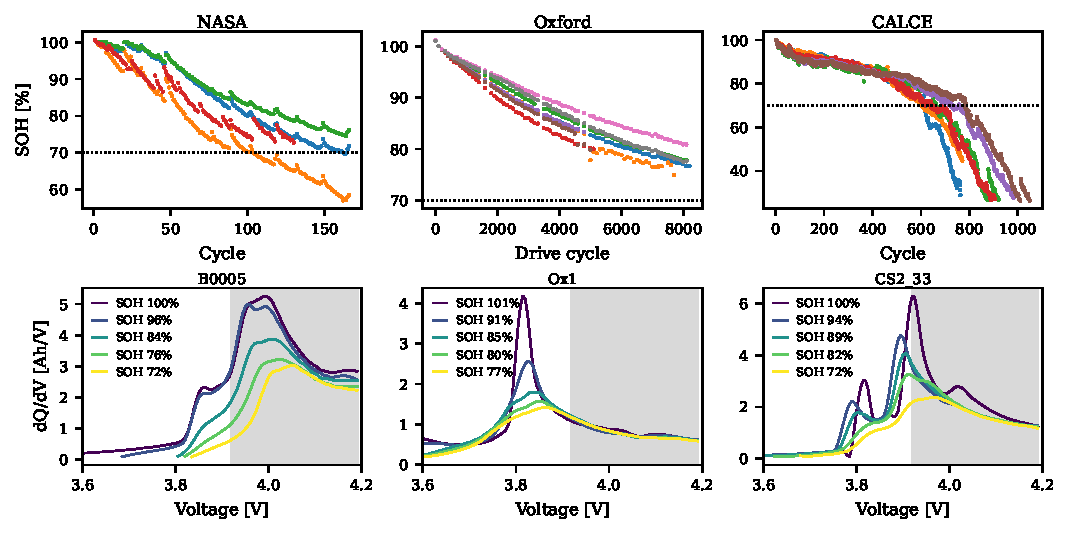
\includegraphics[width=\textwidth]{figures/overview.pdf}
\caption{Top: SOH of every cell (dotted line: 70\% threshold). Bottom: incremental capacity $dQ/dV$ during CC charging for one cell per dataset at increasing age. The shaded area is the common voltage window 3.92--4.19\,V used for the main experiments.}
\label{fig:overview}
\end{figure*}

\section{Methods}
\subsection{Partial-Charge Features}
The CC charge of the NASA and CALCE cells starts at different voltages in different cycles; a window of 3.92--4.19\,V is covered by at least 95\% of the cycles of every dataset and is used unless stated otherwise. For a window $[V_a,V_b]$ we compute nine features: the window charge $\Delta Q=Q(V_b)-Q(V_a)$; the IC curve, smoothed with a Savitzky--Golay filter~\cite{savitzky1964} (11 points, second order), sampled at six equally spaced voltages; and the height and position of the IC maximum within the window. Absolute features are divided by the rated capacity of the cell type.

\subsection{Reference Normalization and Anchoring}
A battery management system can store the charge curve of the first charges of a new cell. Let $\mathbf{f}_{ref}$ be the mean feature vector of the first three cycles of a cell that cover the window. The reference-normalized features are the element-wise ratios $\mathbf{f}/\mathbf{f}_{ref}$, except for the peak position, which is expressed as a shift. The reference cycles are excluded from all training and test sets. The ratio $\Delta Q/\Delta Q_{ref}$ also serves as a training-free SOH estimate, the \emph{capacity ratio}, which is exact if aging scales the charge curve uniformly. We also test \emph{reference anchoring}, $\widehat{\mathrm{SOH}}=g(\mathbf{f})-g(\mathbf{f}_{ref})+1$, which removes any offset of a trained model $g$ at the healthy reference point without using labels of the target cell.

\subsection{Models and Baselines}
We compare ridge regression ($\alpha=1$), GPR with an anisotropic RBF and a white-noise kernel~\cite{rasmussen2006gp} (trained on at most 1{,}500 cycles), a random forest with 300 trees (RF)~\cite{breiman2001rf} and a multilayer perceptron with 64 and 32 units (MLP), all implemented with scikit-learn~\cite{pedregosa2011sklearn}, and gradient-boosted trees with 300 iterations of 15 leaves from the LightGBM library (LGBM)~\cite{ke2017lightgbm}. Inputs of ridge, GPR and MLP are standardized; hyperparameters are fixed. The \emph{cycle-count baseline} uses the cycle number as its only input (ridge and LGBM).

\subsection{Evaluation Protocols}
\begin{itemize}
\item \textbf{Random split:} 80\% of the cycles of a dataset for training, 20\% for testing.
\item \textbf{Leave-one-cell-out (LOCO):} each cell of a dataset is predicted by a model trained on the other cells of the same dataset.
\item \textbf{Leave-one-dataset-out (LODO):} each dataset is predicted by a model trained on the other two. To prevent CALCE from dominating, each training dataset is subsampled to at most 600 cycles.
\end{itemize}
We report the root-mean-square error (RMSE) of SOH in percentage points (pp), the bias and the coefficient of determination $R^2$, computed per dataset over the pooled test predictions.

\section{Results}
\subsection{Effect of the Evaluation Protocol}
Table~\ref{tab:main} lists the RMSE of every configuration, and Fig.~\ref{fig:protocols} summarizes the best configuration of each family averaged over the three datasets. With a random split the best models reach 0.53\,pp (NASA), 0.57\,pp (Oxford) and 1.15\,pp (CALCE), consistent with the sub-percent errors often reported (e.g.,~\cite{roman2021pipeline}). Holding out a cell raises the best errors to 1.50, 1.05 and 2.45\,pp. Holding out a dataset raises them to 6.6\,pp (NASA, achieved by the training-free capacity ratio), 6.5\,pp (Oxford) and 5.9\,pp (CALCE), with $R^2$ values of 0.47, $-0.07$ and 0.26; most other configurations have negative $R^2$, i.e., they are less accurate than predicting the mean SOH of the target dataset. The MLP was unstable on these small training sets (e.g., 37\,pp on Oxford under the random split) and is not discussed further.

\begin{table*}[t]
\caption{RMSE of SOH [percentage points] for every configuration. Columns: test dataset under each protocol. Abs./Ref.: absolute or reference-normalized features.}
\label{tab:main}
\centering
\footnotesize
\begin{tabular}{@{}ll|ccc|ccc|ccc@{}}
\toprule
 & & \multicolumn{3}{c|}{Random split} & \multicolumn{3}{c|}{Leave-one-cell-out} & \multicolumn{3}{c}{Leave-one-dataset-out} \\
Features & Model & NASA & Oxford & CALCE & NASA & Oxford & CALCE & NASA & Oxford & CALCE \\
\midrule
Abs. & Ridge & 1.9 & 1.8 & 2.7 & 4.2 & 2.0 & 4.9 & 32.6 & 8.7 & 27.6 \\
Abs. & GPR & 0.7 & 1.1 & 1.1 & 3.9 & 1.7 & 3.9 & 9.2 & 6.5 & 9.8 \\
Abs. & RF & 1.4 & 1.1 & 1.2 & 3.3 & 1.6 & 2.8 & 16.0 & 14.9 & 12.5 \\
Abs. & LGBM & 1.4 & 1.0 & 1.2 & 3.5 & 1.7 & 2.5 & 16.4 & 14.0 & 13.5 \\
Abs. & MLP & 2.2 & 37.2 & 3.2 & 15.1 & 15.6 & 10.7 & 13.5 & 12.9 & 32.5 \\
\midrule
Ref. & Ridge & 0.8 & 1.0 & 2.5 & 1.5 & 1.2 & 6.9 & 12.7 & 19.3 & 7.3 \\
Ref. & GPR & 0.5 & 0.6 & 1.3 & 4.1 & 1.1 & 4.3 & 8.9 & 9.5 & 6.3 \\
Ref. & RF & 0.8 & 0.7 & 1.2 & 2.8 & 1.1 & 3.4 & 10.3 & 12.5 & 5.9 \\
Ref. & LGBM & 0.7 & 0.7 & 1.3 & 2.6 & 1.2 & 3.3 & 8.3 & 13.2 & 5.9 \\
Ref. & MLP & 1.5 & 3.2 & 3.8 & 21.1 & 18.4 & 12.4 & 29.9 & 17.0 & 20.3 \\
\midrule
Cycle & Ridge & 4.0 & 1.8 & 2.2 & 5.5 & 2.1 & 2.3 & 9.7 & 62.5 & 6.7 \\
Cycle & LGBM & 4.7 & 1.8 & 2.0 & 5.2 & 1.9 & 2.3 & 11.8 & 14.4 & 13.9 \\
\multicolumn{2}{@{}l}{Capacity ratio} & 6.7 & 12.1 & 6.0 & 6.6 & 12.1 & 6.1 & 6.6 & 12.1 & 6.1 \\
\bottomrule
\end{tabular}
\end{table*}

\begin{figure}[t]
\centering
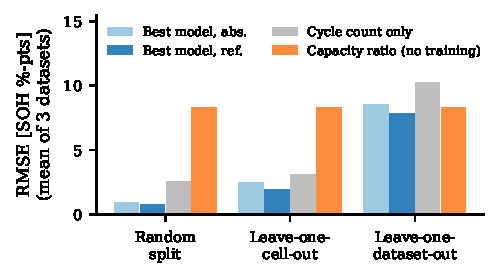
\includegraphics[width=\columnwidth]{figures/protocols.pdf}
\caption{RMSE of the best configuration of each family, averaged over the three test datasets, under the three protocols.}
\label{fig:protocols}
\end{figure}

\subsection{Cycle Count as a Baseline}
Within a dataset, the cells follow the same or similar test procedures, so the cycle number alone carries much of the SOH information. Under LOCO the cycle-count baseline reaches 5.2, 1.9 and 2.3\,pp. On CALCE it is better than every charge-curve model (best 2.45\,pp), and on Oxford it is within 0.9\,pp of the best model. The baseline cannot transfer across datasets, where cycle numbers have different meanings (e.g., Oxford counts drive cycles), and its LODO errors reach 6.8--62.5\,pp. Within a dataset, a charge-curve model adds value only where it outperforms a cycle counter, and reporting this baseline makes that comparison explicit.

\subsection{Reference Normalization}
Within a dataset, reference normalization helps the linear model most: under LOCO, ridge improves from 4.2 to 1.5\,pp on NASA and from 2.0 to 1.2\,pp on Oxford. Across datasets it lowers the error of the tree ensembles on NASA (LGBM: 16.4 to 8.3\,pp; RF: 16.0 to 10.3\,pp) and CALCE (LGBM: 13.5 to 5.9\,pp; RF: 12.5 to 5.9\,pp), but not on Oxford, where the best LODO model uses absolute features (GPR, 6.5\,pp). Averaged over the three datasets, the best reference-normalized configuration has a LODO error of 7.9\,pp compared with 8.5\,pp for absolute features. Reference anchoring did not provide a further benefit: it reduced the error of strongly biased models (ridge with absolute features: NASA 32.6 to 19.4\,pp, CALCE 27.6 to 12.5\,pp) but increased it for most other configurations, and it improved the best LODO error of only one dataset, by 0.04\,pp (CALCE: 5.86 to 5.82\,pp with LGBM).

\subsection{Why Transfer Fails}
Fig.~\ref{fig:ratio} plots the true SOH against the capacity ratio $\Delta Q/\Delta Q_{ref}$. If aging only scaled the charge curve, all points would lie on the diagonal. Instead, the fitted slopes are 0.66 (NASA), 0.77 (CALCE) and 1.56 (Oxford). For the Oxford cells the window charge decreases only to about 95\% of its reference value while SOH decreases to 75\%, so the capacity ratio overestimates SOH by 10.5\,pp on average. Fig.~\ref{fig:overview} suggests a reason: the dominant IC peak of the Oxford cells, which shrinks and shifts with age, lies at about 3.82\,V, below the common window. A shift of the curve along the voltage axis, as caused by loss of lithium inventory~\cite{dubarry2012modes,birkl2017diagnostics}, can change the charge in a high-voltage window less than the total capacity. Because the relation between window features and capacity differs between datasets in slope and not only in offset, a model trained on two datasets is biased on the third, and anchoring at the healthy point cannot correct a slope error. The training-free capacity ratio has the lowest LODO error on NASA (6.6\,pp, bias $-4.2$\,pp), but its errors on the other datasets are 12.2 and 6.1\,pp.

\begin{figure}[t]
\centering
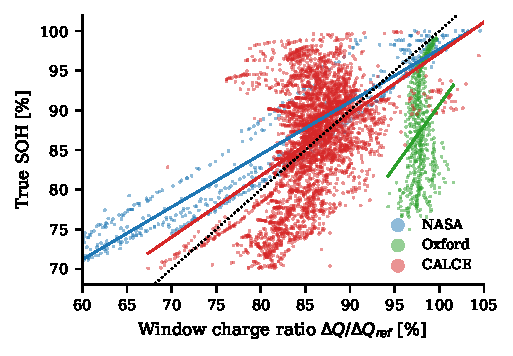
\includegraphics[width=\columnwidth]{figures/ratio.pdf}
\caption{True SOH versus the window charge ratio $\Delta Q/\Delta Q_{ref}$ (3.92--4.19\,V) with a linear fit per dataset. The dotted line is the identity.}
\label{fig:ratio}
\end{figure}

\subsection{Position and Width of the Voltage Window}
Fig.~\ref{fig:windows} shows the mean LODO error for windows of 50--270\,mV at different positions. The window matters more than its width: for LGBM with reference-normalized features the error ranges from 6.8 to 13.7\,pp depending on the position, and several 50\,mV windows near 4.1\,V reach 7.2--7.5\,pp, which is lower than the 9.1\,pp of the full 270\,mV window. The lowest errors were 6.8\,pp (LGBM, 3.95--4.15\,V), 6.3\,pp (ridge, 3.99--4.04\,V) and 7.4\,pp (capacity ratio, 3.99--4.14\,V). Because these windows were selected using the held-out datasets, the minima are optimistic and are reported only to show the sensitivity to the window; a deployed system would have to fix the window in advance.

\begin{figure}[t]
\centering
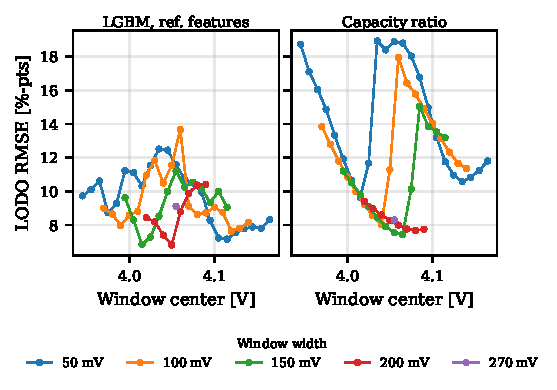
\includegraphics[width=\columnwidth]{figures/windows.pdf}
\caption{Mean leave-one-dataset-out RMSE as a function of the window center for five window widths.}
\label{fig:windows}
\end{figure}

\subsection{Computational Cost}
Feature extraction requires only a differentiation and a few interpolations of the stored charge curve. On a laptop CPU without a GPU, ridge regression needs 1.1\,kB of storage and 0.25\,ms per prediction, the MLP 79\,kB and 0.26\,ms, and LGBM 452\,kB and 0.57\,ms. GPR (21\,MB, 0.37\,ms) stores its training data, and the RF (19\,MB, 50\,ms) stores 300 deep trees.

\section{Discussion}
\textbf{Implications.} Errors obtained with random splits of cycles describe interpolation along known aging trajectories and should not be compared with errors on new cells. Within a dataset, the cycle-count baseline shows how much of the reported accuracy is explained by the shared test procedure. Across datasets, none of the evaluated configurations reached an error below 5.8\,pp, so a model trained on public data should not be expected to work on a different cell type without target data. Reference normalization is a cheap step that lowered the error in 26 of 36 combinations of model, protocol and dataset (excluding the MLP), and its failure on Oxford shows that a common window can miss the voltage range in which a given cell type ages.

\textbf{Limitations.} The benchmark contains 18 cells from three laboratories. Cell type, charge rate, temperature and discharge profile change together between datasets, so their individual effects cannot be separated. SOH is measured with each dataset's own discharge protocol, which adds a systematic difference between datasets. Only CC charging features were used; constant-voltage and temperature features may transfer differently~\cite{le2026charging}. Hyperparameters were not tuned.

\section{Conclusion}
We evaluated partial-charge SOH estimation on three public datasets under three protocols. The mean error of the best models grows from 0.8\,pp with a random split to 2.0\,pp for unseen cells and 7.9\,pp for unseen datasets, where most configurations are worse than predicting the mean. Within a dataset, a cycle counter is a strong baseline: it is the best predictor for held-out CALCE cells and within 0.9\,pp of the best model on Oxford. Reference normalization reduces the cross-dataset error on two of three datasets, but a dataset-dependent relation between window charge and capacity limits transfer. Future work will add datasets with varied temperatures and charge rates and study adaptation with a few labeled cycles of the target cell type.

\section*{Data and Code Availability}
The NASA, Oxford and CALCE datasets are publicly available from their providers~\cite{saha2007nasa,birkl2017oxforddata,calcearchive}. The code that reproduces all experiments, figures and tables is available at \url{https://github.com/shahihussainofficial1/battery-soh-transfer}.

\bibliographystyle{IEEEtran}
\bibliography{references}

\end{document}
